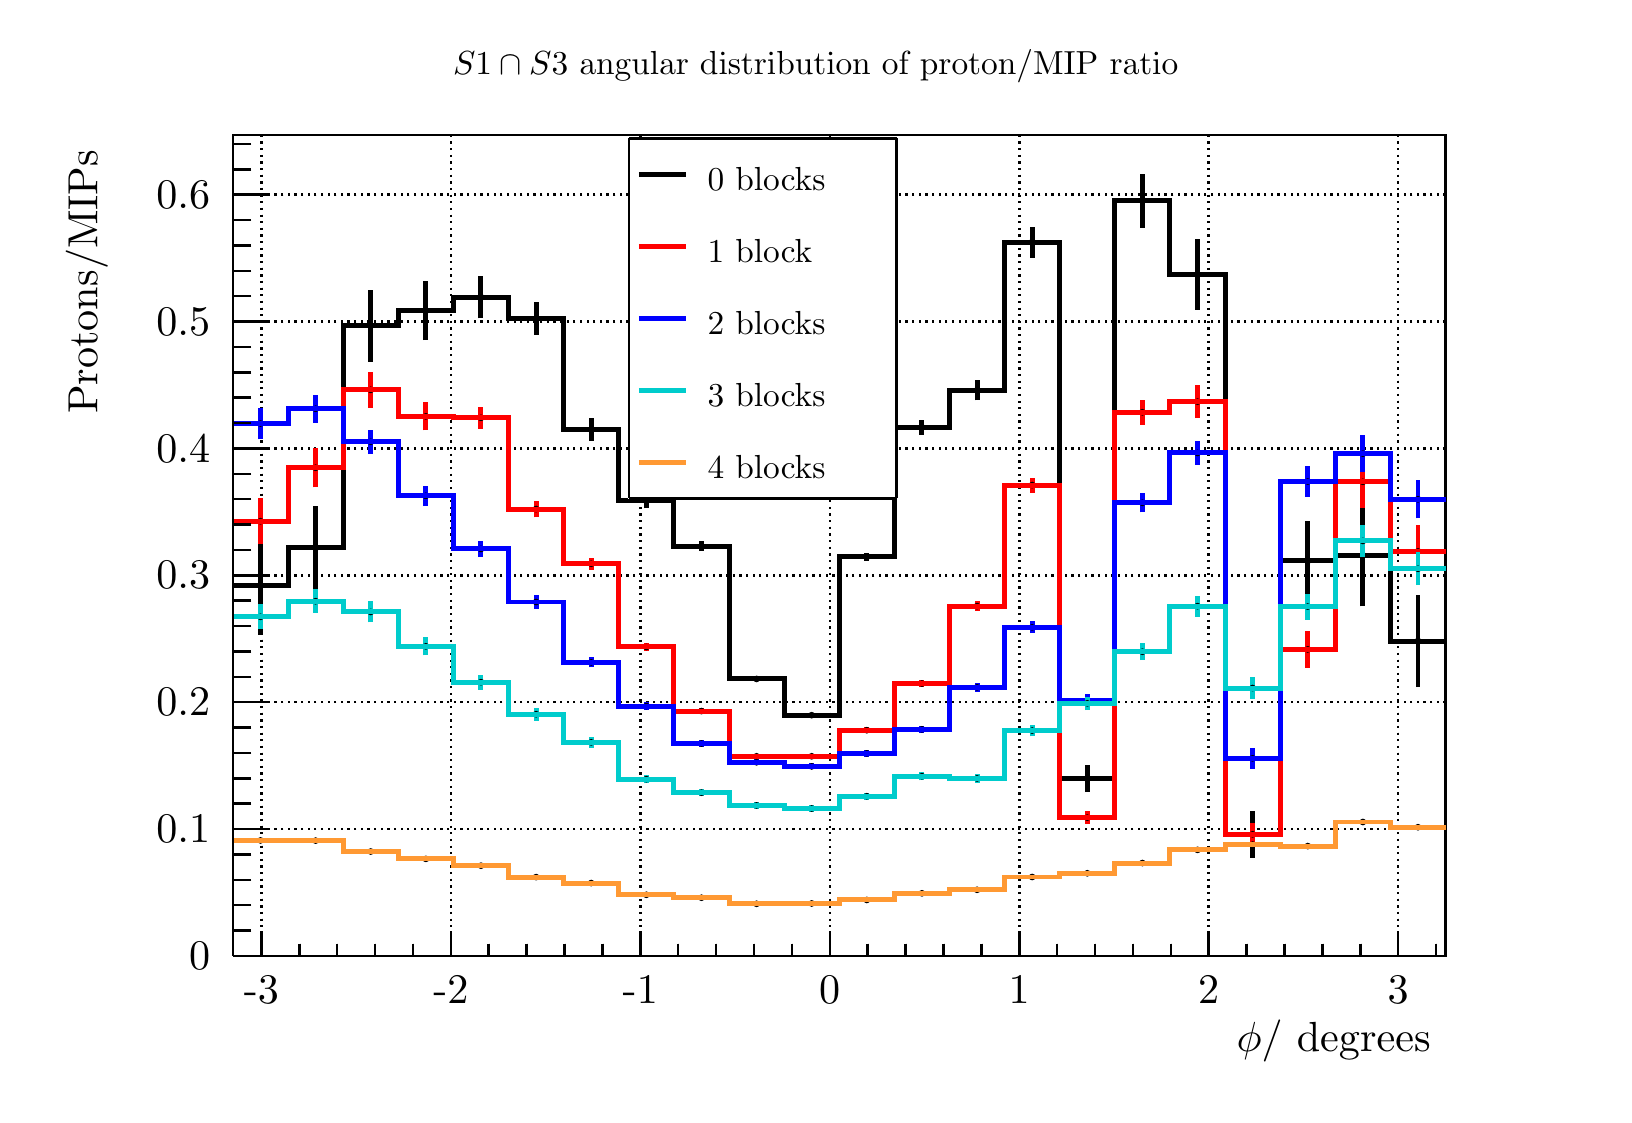
\begin{tikzpicture}
\pgfdeclareplotmark{cross} {
\pgfpathmoveto{\pgfpoint{-0.3\pgfplotmarksize}{\pgfplotmarksize}}
\pgfpathlineto{\pgfpoint{+0.3\pgfplotmarksize}{\pgfplotmarksize}}
\pgfpathlineto{\pgfpoint{+0.3\pgfplotmarksize}{0.3\pgfplotmarksize}}
\pgfpathlineto{\pgfpoint{+1\pgfplotmarksize}{0.3\pgfplotmarksize}}
\pgfpathlineto{\pgfpoint{+1\pgfplotmarksize}{-0.3\pgfplotmarksize}}
\pgfpathlineto{\pgfpoint{+0.3\pgfplotmarksize}{-0.3\pgfplotmarksize}}
\pgfpathlineto{\pgfpoint{+0.3\pgfplotmarksize}{-1.\pgfplotmarksize}}
\pgfpathlineto{\pgfpoint{-0.3\pgfplotmarksize}{-1.\pgfplotmarksize}}
\pgfpathlineto{\pgfpoint{-0.3\pgfplotmarksize}{-0.3\pgfplotmarksize}}
\pgfpathlineto{\pgfpoint{-1.\pgfplotmarksize}{-0.3\pgfplotmarksize}}
\pgfpathlineto{\pgfpoint{-1.\pgfplotmarksize}{0.3\pgfplotmarksize}}
\pgfpathlineto{\pgfpoint{-0.3\pgfplotmarksize}{0.3\pgfplotmarksize}}
\pgfpathclose
\pgfusepathqstroke
}
\pgfdeclareplotmark{cross*} {
\pgfpathmoveto{\pgfpoint{-0.3\pgfplotmarksize}{\pgfplotmarksize}}
\pgfpathlineto{\pgfpoint{+0.3\pgfplotmarksize}{\pgfplotmarksize}}
\pgfpathlineto{\pgfpoint{+0.3\pgfplotmarksize}{0.3\pgfplotmarksize}}
\pgfpathlineto{\pgfpoint{+1\pgfplotmarksize}{0.3\pgfplotmarksize}}
\pgfpathlineto{\pgfpoint{+1\pgfplotmarksize}{-0.3\pgfplotmarksize}}
\pgfpathlineto{\pgfpoint{+0.3\pgfplotmarksize}{-0.3\pgfplotmarksize}}
\pgfpathlineto{\pgfpoint{+0.3\pgfplotmarksize}{-1.\pgfplotmarksize}}
\pgfpathlineto{\pgfpoint{-0.3\pgfplotmarksize}{-1.\pgfplotmarksize}}
\pgfpathlineto{\pgfpoint{-0.3\pgfplotmarksize}{-0.3\pgfplotmarksize}}
\pgfpathlineto{\pgfpoint{-1.\pgfplotmarksize}{-0.3\pgfplotmarksize}}
\pgfpathlineto{\pgfpoint{-1.\pgfplotmarksize}{0.3\pgfplotmarksize}}
\pgfpathlineto{\pgfpoint{-0.3\pgfplotmarksize}{0.3\pgfplotmarksize}}
\pgfpathclose
\pgfusepathqfillstroke
}
\pgfdeclareplotmark{newstar} {
\pgfpathmoveto{\pgfqpoint{0pt}{\pgfplotmarksize}}
\pgfpathlineto{\pgfqpointpolar{44}{0.5\pgfplotmarksize}}
\pgfpathlineto{\pgfqpointpolar{18}{\pgfplotmarksize}}
\pgfpathlineto{\pgfqpointpolar{-20}{0.5\pgfplotmarksize}}
\pgfpathlineto{\pgfqpointpolar{-54}{\pgfplotmarksize}}
\pgfpathlineto{\pgfqpointpolar{-90}{0.5\pgfplotmarksize}}
\pgfpathlineto{\pgfqpointpolar{234}{\pgfplotmarksize}}
\pgfpathlineto{\pgfqpointpolar{198}{0.5\pgfplotmarksize}}
\pgfpathlineto{\pgfqpointpolar{162}{\pgfplotmarksize}}
\pgfpathlineto{\pgfqpointpolar{134}{0.5\pgfplotmarksize}}
\pgfpathclose
\pgfusepathqstroke
}
\pgfdeclareplotmark{newstar*} {
\pgfpathmoveto{\pgfqpoint{0pt}{\pgfplotmarksize}}
\pgfpathlineto{\pgfqpointpolar{44}{0.5\pgfplotmarksize}}
\pgfpathlineto{\pgfqpointpolar{18}{\pgfplotmarksize}}
\pgfpathlineto{\pgfqpointpolar{-20}{0.5\pgfplotmarksize}}
\pgfpathlineto{\pgfqpointpolar{-54}{\pgfplotmarksize}}
\pgfpathlineto{\pgfqpointpolar{-90}{0.5\pgfplotmarksize}}
\pgfpathlineto{\pgfqpointpolar{234}{\pgfplotmarksize}}
\pgfpathlineto{\pgfqpointpolar{198}{0.5\pgfplotmarksize}}
\pgfpathlineto{\pgfqpointpolar{162}{\pgfplotmarksize}}
\pgfpathlineto{\pgfqpointpolar{134}{0.5\pgfplotmarksize}}
\pgfpathclose
\pgfusepathqfillstroke
}
\definecolor{c}{rgb}{1,1,1};
\draw [color=c, fill=c] (0,0) rectangle (20,13.5429);
\draw [color=c, fill=c] (2.6,1.76057) rectangle (18,12.1886);
\definecolor{c}{rgb}{0,0,0};
\draw [c,line width=0.9] (2.6,1.76057) -- (2.6,12.1886) -- (18,12.1886) -- (18,1.76057) -- (2.6,1.76057);
\definecolor{c}{rgb}{1,1,1};
\draw [color=c, fill=c] (2.6,1.76057) rectangle (18,12.1886);
\definecolor{c}{rgb}{0,0,0};
\draw [c,line width=0.9] (2.6,1.76057) -- (2.6,12.1886) -- (18,12.1886) -- (18,1.76057) -- (2.6,1.76057);
\draw [c,line width=0.9] (2.6,1.76057) -- (18,1.76057);
\draw [c,dash pattern=on 0.80pt off 1.60pt ,line width=0.9] (2.96094,12.1886) -- (2.96094,1.76057);
\draw [c,dash pattern=on 0.80pt off 1.60pt ,line width=0.9] (5.36719,12.1886) -- (5.36719,1.76057);
\draw [c,dash pattern=on 0.80pt off 1.60pt ,line width=0.9] (7.77344,12.1886) -- (7.77344,1.76057);
\draw [c,dash pattern=on 0.80pt off 1.60pt ,line width=0.9] (10.1797,12.1886) -- (10.1797,1.76057);
\draw [c,dash pattern=on 0.80pt off 1.60pt ,line width=0.9] (12.5859,12.1886) -- (12.5859,1.76057);
\draw [c,dash pattern=on 0.80pt off 1.60pt ,line width=0.9] (14.9922,12.1886) -- (14.9922,1.76057);
\draw [c,dash pattern=on 0.80pt off 1.60pt ,line width=0.9] (17.3984,12.1886) -- (17.3984,1.76057);
\draw [c,dash pattern=on 0.80pt off 1.60pt ,line width=0.9] (2.96094,12.1886) -- (2.96094,1.76057);
\draw [c,dash pattern=on 0.80pt off 1.60pt ,line width=0.9] (17.3984,12.1886) -- (17.3984,1.76057);
\draw [c,line width=0.9] (2.6,1.76057) -- (2.6,12.1886);
\draw [c,dash pattern=on 0.80pt off 1.60pt ,line width=0.9] (18,1.76057) -- (2.6,1.76057);
\draw [c,dash pattern=on 0.80pt off 1.60pt ,line width=0.9] (18,3.3719) -- (2.6,3.3719);
\draw [c,dash pattern=on 0.80pt off 1.60pt ,line width=0.9] (18,4.98322) -- (2.6,4.98322);
\draw [c,dash pattern=on 0.80pt off 1.60pt ,line width=0.9] (18,6.59455) -- (2.6,6.59455);
\draw [c,dash pattern=on 0.80pt off 1.60pt ,line width=0.9] (18,8.20588) -- (2.6,8.20588);
\draw [c,dash pattern=on 0.80pt off 1.60pt ,line width=0.9] (18,9.8172) -- (2.6,9.8172);
\draw [c,dash pattern=on 0.80pt off 1.60pt ,line width=0.9] (18,11.4285) -- (2.6,11.4285);
\draw [c,dash pattern=on 0.80pt off 1.60pt ,line width=0.9] (18,11.4285) -- (2.6,11.4285);
\definecolor{c}{rgb}{0,0,0.6};
\draw [c,line width=0.9] (2.6,1.76057) -- (3.3,1.76057) -- (3.3,1.76057) -- (4,1.76057) -- (4,1.76057) -- (4.7,1.76057) -- (4.7,1.76057) -- (5.4,1.76057) -- (5.4,1.76057) -- (6.1,1.76057) -- (6.1,1.76057) -- (6.8,1.76057) -- (6.8,1.76057) --
 (7.5,1.76057) -- (7.5,1.76057) -- (8.2,1.76057) -- (8.2,1.76057) -- (8.9,1.76057) -- (8.9,1.76057) -- (9.6,1.76057) -- (9.6,1.76057) -- (10.3,1.76057) -- (10.3,1.76057) -- (11,1.76057) -- (11,1.76057) -- (11.7,1.76057) -- (11.7,1.76057) --
 (12.4,1.76057) -- (12.4,1.76057) -- (13.1,1.76057) -- (13.1,1.76057) -- (13.8,1.76057) -- (13.8,1.76057) -- (14.5,1.76057) -- (14.5,1.76057) -- (15.2,1.76057) -- (15.2,1.76057) -- (15.9,1.76057) -- (15.9,1.76057) -- (16.6,1.76057) -- (16.6,1.76057)
 -- (17.3,1.76057) -- (17.3,1.76057) -- (18,1.76057);
\definecolor{c}{rgb}{0,0,0};
\draw [c,line width=0.9] (2.6,1.76057) -- (18,1.76057);
\draw [c,line width=0.9] (2.96094,2.07341) -- (2.96094,1.76057);
\draw [c,line width=0.9] (3.44219,1.91699) -- (3.44219,1.76057);
\draw [c,line width=0.9] (3.92344,1.91699) -- (3.92344,1.76057);
\draw [c,line width=0.9] (4.40469,1.91699) -- (4.40469,1.76057);
\draw [c,line width=0.9] (4.88594,1.91699) -- (4.88594,1.76057);
\draw [c,line width=0.9] (5.36719,2.07341) -- (5.36719,1.76057);
\draw [c,line width=0.9] (5.84844,1.91699) -- (5.84844,1.76057);
\draw [c,line width=0.9] (6.32969,1.91699) -- (6.32969,1.76057);
\draw [c,line width=0.9] (6.81094,1.91699) -- (6.81094,1.76057);
\draw [c,line width=0.9] (7.29219,1.91699) -- (7.29219,1.76057);
\draw [c,line width=0.9] (7.77344,2.07341) -- (7.77344,1.76057);
\draw [c,line width=0.9] (8.25469,1.91699) -- (8.25469,1.76057);
\draw [c,line width=0.9] (8.73594,1.91699) -- (8.73594,1.76057);
\draw [c,line width=0.9] (9.21719,1.91699) -- (9.21719,1.76057);
\draw [c,line width=0.9] (9.69844,1.91699) -- (9.69844,1.76057);
\draw [c,line width=0.9] (10.1797,2.07341) -- (10.1797,1.76057);
\draw [c,line width=0.9] (10.6609,1.91699) -- (10.6609,1.76057);
\draw [c,line width=0.9] (11.1422,1.91699) -- (11.1422,1.76057);
\draw [c,line width=0.9] (11.6234,1.91699) -- (11.6234,1.76057);
\draw [c,line width=0.9] (12.1047,1.91699) -- (12.1047,1.76057);
\draw [c,line width=0.9] (12.5859,2.07341) -- (12.5859,1.76057);
\draw [c,line width=0.9] (13.0672,1.91699) -- (13.0672,1.76057);
\draw [c,line width=0.9] (13.5484,1.91699) -- (13.5484,1.76057);
\draw [c,line width=0.9] (14.0297,1.91699) -- (14.0297,1.76057);
\draw [c,line width=0.9] (14.5109,1.91699) -- (14.5109,1.76057);
\draw [c,line width=0.9] (14.9922,2.07341) -- (14.9922,1.76057);
\draw [c,line width=0.9] (15.4734,1.91699) -- (15.4734,1.76057);
\draw [c,line width=0.9] (15.9547,1.91699) -- (15.9547,1.76057);
\draw [c,line width=0.9] (16.4359,1.91699) -- (16.4359,1.76057);
\draw [c,line width=0.9] (16.9172,1.91699) -- (16.9172,1.76057);
\draw [c,line width=0.9] (17.3984,2.07341) -- (17.3984,1.76057);
\draw [c,line width=0.9] (2.96094,2.07341) -- (2.96094,1.76057);
\draw [c,line width=0.9] (17.3984,2.07341) -- (17.3984,1.76057);
\draw [c,line width=0.9] (17.8797,1.91699) -- (17.8797,1.76057);
\draw [anchor=base] (2.96094,1.15114) node[scale=1.52295, color=c, rotate=0]{-3};
\draw [anchor=base] (5.36719,1.15114) node[scale=1.52295, color=c, rotate=0]{-2};
\draw [anchor=base] (7.77344,1.15114) node[scale=1.52295, color=c, rotate=0]{-1};
\draw [anchor=base] (10.1797,1.15114) node[scale=1.52295, color=c, rotate=0]{0};
\draw [anchor=base] (12.5859,1.15114) node[scale=1.52295, color=c, rotate=0]{1};
\draw [anchor=base] (14.9922,1.15114) node[scale=1.52295, color=c, rotate=0]{2};
\draw [anchor=base] (17.3984,1.15114) node[scale=1.52295, color=c, rotate=0]{3};
\draw [anchor= east] (18,0.677143) node[scale=1.52295, color=c, rotate=0]{$ \phi $/ degrees};
\draw [c,line width=0.9] (2.6,1.76057) -- (2.6,12.1886);
\draw [c,line width=0.9] (3.062,1.76057) -- (2.6,1.76057);
\draw [c,line width=0.9] (2.831,2.08284) -- (2.6,2.08284);
\draw [c,line width=0.9] (2.831,2.4051) -- (2.6,2.4051);
\draw [c,line width=0.9] (2.831,2.72737) -- (2.6,2.72737);
\draw [c,line width=0.9] (2.831,3.04963) -- (2.6,3.04963);
\draw [c,line width=0.9] (3.062,3.3719) -- (2.6,3.3719);
\draw [c,line width=0.9] (2.831,3.69416) -- (2.6,3.69416);
\draw [c,line width=0.9] (2.831,4.01643) -- (2.6,4.01643);
\draw [c,line width=0.9] (2.831,4.33869) -- (2.6,4.33869);
\draw [c,line width=0.9] (2.831,4.66096) -- (2.6,4.66096);
\draw [c,line width=0.9] (3.062,4.98322) -- (2.6,4.98322);
\draw [c,line width=0.9] (2.831,5.30549) -- (2.6,5.30549);
\draw [c,line width=0.9] (2.831,5.62775) -- (2.6,5.62775);
\draw [c,line width=0.9] (2.831,5.95002) -- (2.6,5.95002);
\draw [c,line width=0.9] (2.831,6.27228) -- (2.6,6.27228);
\draw [c,line width=0.9] (3.062,6.59455) -- (2.6,6.59455);
\draw [c,line width=0.9] (2.831,6.91681) -- (2.6,6.91681);
\draw [c,line width=0.9] (2.831,7.23908) -- (2.6,7.23908);
\draw [c,line width=0.9] (2.831,7.56134) -- (2.6,7.56134);
\draw [c,line width=0.9] (2.831,7.88361) -- (2.6,7.88361);
\draw [c,line width=0.9] (3.062,8.20588) -- (2.6,8.20588);
\draw [c,line width=0.9] (2.831,8.52814) -- (2.6,8.52814);
\draw [c,line width=0.9] (2.831,8.85041) -- (2.6,8.85041);
\draw [c,line width=0.9] (2.831,9.17267) -- (2.6,9.17267);
\draw [c,line width=0.9] (2.831,9.49494) -- (2.6,9.49494);
\draw [c,line width=0.9] (3.062,9.8172) -- (2.6,9.8172);
\draw [c,line width=0.9] (2.831,10.1395) -- (2.6,10.1395);
\draw [c,line width=0.9] (2.831,10.4617) -- (2.6,10.4617);
\draw [c,line width=0.9] (2.831,10.784) -- (2.6,10.784);
\draw [c,line width=0.9] (2.831,11.1063) -- (2.6,11.1063);
\draw [c,line width=0.9] (3.062,11.4285) -- (2.6,11.4285);
\draw [c,line width=0.9] (3.062,11.4285) -- (2.6,11.4285);
\draw [c,line width=0.9] (2.831,11.7508) -- (2.6,11.7508);
\draw [c,line width=0.9] (2.831,12.0731) -- (2.6,12.0731);
\draw [anchor= east] (2.5,1.76057) node[scale=1.52295, color=c, rotate=0]{0};
\draw [anchor= east] (2.5,3.3719) node[scale=1.52295, color=c, rotate=0]{0.1};
\draw [anchor= east] (2.5,4.98322) node[scale=1.52295, color=c, rotate=0]{0.2};
\draw [anchor= east] (2.5,6.59455) node[scale=1.52295, color=c, rotate=0]{0.3};
\draw [anchor= east] (2.5,8.20588) node[scale=1.52295, color=c, rotate=0]{0.4};
\draw [anchor= east] (2.5,9.8172) node[scale=1.52295, color=c, rotate=0]{0.5};
\draw [anchor= east] (2.5,11.4285) node[scale=1.52295, color=c, rotate=0]{0.6};
\draw [anchor= east] (0.742857,12.1886) node[scale=1.52295, color=c, rotate=90]{  Protons/MIPs};
\draw [c,line width=1.8] (2.95,5.83925) -- (2.95,6.46517);
\draw [c,line width=1.8] (2.95,6.46517) -- (2.95,7.09109);
\foreach \P in {(2.95,6.46517)}{\draw[mark options={color=c,fill=c},mark size=2.402402pt,mark=*,mark size=1pt] plot coordinates {\P};}
\draw [c,line width=1.8] (3.65,6.40919) -- (3.65,6.94273);
\draw [c,line width=1.8] (3.65,6.94273) -- (3.65,7.47626);
\foreach \P in {(3.65,6.94273)}{\draw[mark options={color=c,fill=c},mark size=2.402402pt,mark=*,mark size=1pt] plot coordinates {\P};}
\draw [c,line width=1.8] (4.35,9.30945) -- (4.35,9.76556);
\draw [c,line width=1.8] (4.35,9.76556) -- (4.35,10.2217);
\foreach \P in {(4.35,9.76556)}{\draw[mark options={color=c,fill=c},mark size=2.402402pt,mark=*,mark size=1pt] plot coordinates {\P};}
\draw [c,line width=1.8] (5.05,9.58256) -- (5.05,9.95492);
\draw [c,line width=1.8] (5.05,9.95492) -- (5.05,10.3273);
\foreach \P in {(5.05,9.95492)}{\draw[mark options={color=c,fill=c},mark size=2.402402pt,mark=*,mark size=1pt] plot coordinates {\P};}
\draw [c,line width=1.8] (5.75,9.85709) -- (5.75,10.1285);
\draw [c,line width=1.8] (5.75,10.1285) -- (5.75,10.3999);
\foreach \P in {(5.75,10.1285)}{\draw[mark options={color=c,fill=c},mark size=2.402402pt,mark=*,mark size=1pt] plot coordinates {\P};}
\draw [c,line width=1.8] (6.45,9.64718) -- (6.45,9.85457);
\draw [c,line width=1.8] (6.45,9.85457) -- (6.45,10.062);
\foreach \P in {(6.45,9.85457)}{\draw[mark options={color=c,fill=c},mark size=2.402402pt,mark=*,mark size=1pt] plot coordinates {\P};}
\draw [c,line width=1.8] (7.15,8.30457) -- (7.15,8.44591);
\draw [c,line width=1.8] (7.15,8.44591) -- (7.15,8.58726);
\foreach \P in {(7.15,8.44591)}{\draw[mark options={color=c,fill=c},mark size=2.402402pt,mark=*,mark size=1pt] plot coordinates {\P};}
\draw [c,line width=1.8] (7.85,7.44584) -- (7.85,7.54129);
\draw [c,line width=1.8] (7.85,7.54129) -- (7.85,7.63674);
\foreach \P in {(7.85,7.54129)}{\draw[mark options={color=c,fill=c},mark size=2.402402pt,mark=*,mark size=1pt] plot coordinates {\P};}
\draw [c,line width=1.8] (8.55,6.90339) -- (8.55,6.96563);
\draw [c,line width=1.8] (8.55,6.96563) -- (8.55,7.02788);
\foreach \P in {(8.55,6.96563)}{\draw[mark options={color=c,fill=c},mark size=2.402402pt,mark=*,mark size=1pt] plot coordinates {\P};}
\draw [c,line width=1.8] (9.25,5.2471) -- (9.25,5.27876);
\draw [c,line width=1.8] (9.25,5.27876) -- (9.25,5.31041);
\foreach \P in {(9.25,5.27876)}{\draw[mark options={color=c,fill=c},mark size=2.402402pt,mark=*,mark size=1pt] plot coordinates {\P};}
\draw [c,line width=1.8] (9.95,4.79237) -- (9.95,4.81847);
\draw [c,line width=1.8] (9.95,4.81847) -- (9.95,4.84458);
\foreach \P in {(9.95,4.81847)}{\draw[mark options={color=c,fill=c},mark size=2.402402pt,mark=*,mark size=1pt] plot coordinates {\P};}
\draw [c,line width=1.8] (10.65,6.77753) -- (10.65,6.82904);
\draw [c,line width=1.8] (10.65,6.82904) -- (10.65,6.88054);
\foreach \P in {(10.65,6.82904)}{\draw[mark options={color=c,fill=c},mark size=2.402402pt,mark=*,mark size=1pt] plot coordinates {\P};}
\draw [c,line width=1.8] (11.35,8.38211) -- (11.35,8.47371);
\draw [c,line width=1.8] (11.35,8.47371) -- (11.35,8.56532);
\foreach \P in {(11.35,8.47371)}{\draw[mark options={color=c,fill=c},mark size=2.402402pt,mark=*,mark size=1pt] plot coordinates {\P};}
\draw [c,line width=1.8] (12.05,8.81727) -- (12.05,8.94467);
\draw [c,line width=1.8] (12.05,8.94467) -- (12.05,9.07207);
\foreach \P in {(12.05,8.94467)}{\draw[mark options={color=c,fill=c},mark size=2.402402pt,mark=*,mark size=1pt] plot coordinates {\P};}
\draw [c,line width=1.8] (12.75,10.6294) -- (12.75,10.8255);
\draw [c,line width=1.8] (12.75,10.8255) -- (12.75,11.0216);
\foreach \P in {(12.75,10.8255)}{\draw[mark options={color=c,fill=c},mark size=2.402402pt,mark=*,mark size=1pt] plot coordinates {\P};}
\draw [c,line width=1.8] (13.45,3.84167) -- (13.45,4.0128);
\draw [c,line width=1.8] (13.45,4.0128) -- (13.45,4.18393);
\foreach \P in {(13.45,4.0128)}{\draw[mark options={color=c,fill=c},mark size=2.402402pt,mark=*,mark size=1pt] plot coordinates {\P};}
\draw [c,line width=1.8] (14.15,11.0087) -- (14.15,11.3504);
\draw [c,line width=1.8] (14.15,11.3504) -- (14.15,11.692);
\foreach \P in {(14.15,11.3504)}{\draw[mark options={color=c,fill=c},mark size=2.402402pt,mark=*,mark size=1pt] plot coordinates {\P};}
\draw [c,line width=1.8] (14.85,9.96997) -- (14.85,10.4177);
\draw [c,line width=1.8] (14.85,10.4177) -- (14.85,10.8654);
\foreach \P in {(14.85,10.4177)}{\draw[mark options={color=c,fill=c},mark size=2.402402pt,mark=*,mark size=1pt] plot coordinates {\P};}
\draw [c,line width=1.8] (15.55,3.00723) -- (15.55,3.30744);
\draw [c,line width=1.8] (15.55,3.30744) -- (15.55,3.60766);
\foreach \P in {(15.55,3.30744)}{\draw[mark options={color=c,fill=c},mark size=2.402402pt,mark=*,mark size=1pt] plot coordinates {\P};}
\draw [c,line width=1.8] (16.25,6.26454) -- (16.25,6.77696);
\draw [c,line width=1.8] (16.25,6.77696) -- (16.25,7.28939);
\foreach \P in {(16.25,6.77696)}{\draw[mark options={color=c,fill=c},mark size=2.402402pt,mark=*,mark size=1pt] plot coordinates {\P};}
\draw [c,line width=1.8] (16.95,6.19951) -- (16.95,6.84897);
\draw [c,line width=1.8] (16.95,6.84897) -- (16.95,7.49843);
\foreach \P in {(16.95,6.84897)}{\draw[mark options={color=c,fill=c},mark size=2.402402pt,mark=*,mark size=1pt] plot coordinates {\P};}
\draw [c,line width=1.8] (17.65,5.17412) -- (17.65,5.76032);
\draw [c,line width=1.8] (17.65,5.76032) -- (17.65,6.34651);
\foreach \P in {(17.65,5.76032)}{\draw[mark options={color=c,fill=c},mark size=2.402402pt,mark=*,mark size=1pt] plot coordinates {\P};}
\draw [c,line width=1.8] (2.6,6.46517) -- (3.3,6.46517) -- (3.3,6.94273) -- (4,6.94273) -- (4,9.76556) -- (4.7,9.76556) -- (4.7,9.95492) -- (5.4,9.95492) -- (5.4,10.1285) -- (6.1,10.1285) -- (6.1,9.85457) -- (6.8,9.85457) -- (6.8,8.44591) --
 (7.5,8.44591) -- (7.5,7.54129) -- (8.2,7.54129) -- (8.2,6.96563) -- (8.9,6.96563) -- (8.9,5.27876) -- (9.6,5.27876) -- (9.6,4.81847) -- (10.3,4.81847) -- (10.3,6.82904) -- (11,6.82904) -- (11,8.47371) -- (11.7,8.47371) -- (11.7,8.94467) --
 (12.4,8.94467) -- (12.4,10.8255) -- (13.1,10.8255) -- (13.1,4.0128) -- (13.8,4.0128) -- (13.8,11.3504) -- (14.5,11.3504) -- (14.5,10.4177) -- (15.2,10.4177) -- (15.2,3.30744) -- (15.9,3.30744) -- (15.9,6.77696) -- (16.6,6.77696) -- (16.6,6.84897) --
 (17.3,6.84897) -- (17.3,5.76032) -- (18,5.76032);
\definecolor{c}{rgb}{1,0,0};
\draw [c,line width=1.8] (2.95,6.98847) -- (2.95,7.28173);
\draw [c,line width=1.8] (2.95,7.28173) -- (2.95,7.57499);
\definecolor{c}{rgb}{0,0,0};
\foreach \P in {(2.95,7.28173)}{\draw[mark options={color=c,fill=c},mark size=2.402402pt,mark=*,mark size=1pt] plot coordinates {\P};}
\definecolor{c}{rgb}{1,0,0};
\draw [c,line width=1.8] (3.65,7.7107) -- (3.65,7.9605);
\draw [c,line width=1.8] (3.65,7.9605) -- (3.65,8.21029);
\definecolor{c}{rgb}{0,0,0};
\foreach \P in {(3.65,7.9605)}{\draw[mark options={color=c,fill=c},mark size=2.402402pt,mark=*,mark size=1pt] plot coordinates {\P};}
\definecolor{c}{rgb}{1,0,0};
\draw [c,line width=1.8] (4.35,8.72565) -- (4.35,8.95015);
\draw [c,line width=1.8] (4.35,8.95015) -- (4.35,9.17464);
\definecolor{c}{rgb}{0,0,0};
\foreach \P in {(4.35,8.95015)}{\draw[mark options={color=c,fill=c},mark size=2.402402pt,mark=*,mark size=1pt] plot coordinates {\P};}
\definecolor{c}{rgb}{1,0,0};
\draw [c,line width=1.8] (5.05,8.43475) -- (5.05,8.61315);
\draw [c,line width=1.8] (5.05,8.61315) -- (5.05,8.79155);
\definecolor{c}{rgb}{0,0,0};
\foreach \P in {(5.05,8.61315)}{\draw[mark options={color=c,fill=c},mark size=2.402402pt,mark=*,mark size=1pt] plot coordinates {\P};}
\definecolor{c}{rgb}{1,0,0};
\draw [c,line width=1.8] (5.75,8.45487) -- (5.75,8.59499);
\draw [c,line width=1.8] (5.75,8.59499) -- (5.75,8.73511);
\definecolor{c}{rgb}{0,0,0};
\foreach \P in {(5.75,8.59499)}{\draw[mark options={color=c,fill=c},mark size=2.402402pt,mark=*,mark size=1pt] plot coordinates {\P};}
\definecolor{c}{rgb}{1,0,0};
\draw [c,line width=1.8] (6.45,7.33048) -- (6.45,7.43631);
\draw [c,line width=1.8] (6.45,7.43631) -- (6.45,7.54215);
\definecolor{c}{rgb}{0,0,0};
\foreach \P in {(6.45,7.43631)}{\draw[mark options={color=c,fill=c},mark size=2.402402pt,mark=*,mark size=1pt] plot coordinates {\P};}
\definecolor{c}{rgb}{1,0,0};
\draw [c,line width=1.8] (7.15,6.66607) -- (7.15,6.74155);
\draw [c,line width=1.8] (7.15,6.74155) -- (7.15,6.81702);
\definecolor{c}{rgb}{0,0,0};
\foreach \P in {(7.15,6.74155)}{\draw[mark options={color=c,fill=c},mark size=2.402402pt,mark=*,mark size=1pt] plot coordinates {\P};}
\definecolor{c}{rgb}{1,0,0};
\draw [c,line width=1.8] (7.85,5.63172) -- (7.85,5.68478);
\draw [c,line width=1.8] (7.85,5.68478) -- (7.85,5.73785);
\definecolor{c}{rgb}{0,0,0};
\foreach \P in {(7.85,5.68478)}{\draw[mark options={color=c,fill=c},mark size=2.402402pt,mark=*,mark size=1pt] plot coordinates {\P};}
\definecolor{c}{rgb}{1,0,0};
\draw [c,line width=1.8] (8.55,4.83176) -- (8.55,4.87056);
\draw [c,line width=1.8] (8.55,4.87056) -- (8.55,4.90936);
\definecolor{c}{rgb}{0,0,0};
\foreach \P in {(8.55,4.87056)}{\draw[mark options={color=c,fill=c},mark size=2.402402pt,mark=*,mark size=1pt] plot coordinates {\P};}
\definecolor{c}{rgb}{1,0,0};
\draw [c,line width=1.8] (9.25,4.2655) -- (9.25,4.29637);
\draw [c,line width=1.8] (9.25,4.29637) -- (9.25,4.32724);
\definecolor{c}{rgb}{0,0,0};
\foreach \P in {(9.25,4.29637)}{\draw[mark options={color=c,fill=c},mark size=2.402402pt,mark=*,mark size=1pt] plot coordinates {\P};}
\definecolor{c}{rgb}{1,0,0};
\draw [c,line width=1.8] (9.95,4.26628) -- (9.95,4.29658);
\draw [c,line width=1.8] (9.95,4.29658) -- (9.95,4.32689);
\definecolor{c}{rgb}{0,0,0};
\foreach \P in {(9.95,4.29658)}{\draw[mark options={color=c,fill=c},mark size=2.402402pt,mark=*,mark size=1pt] plot coordinates {\P};}
\definecolor{c}{rgb}{1,0,0};
\draw [c,line width=1.8] (10.65,4.59295) -- (10.65,4.62766);
\draw [c,line width=1.8] (10.65,4.62766) -- (10.65,4.66237);
\definecolor{c}{rgb}{0,0,0};
\foreach \P in {(10.65,4.62766)}{\draw[mark options={color=c,fill=c},mark size=2.402402pt,mark=*,mark size=1pt] plot coordinates {\P};}
\definecolor{c}{rgb}{1,0,0};
\draw [c,line width=1.8] (11.35,5.17534) -- (11.35,5.2201);
\draw [c,line width=1.8] (11.35,5.2201) -- (11.35,5.26486);
\definecolor{c}{rgb}{0,0,0};
\foreach \P in {(11.35,5.2201)}{\draw[mark options={color=c,fill=c},mark size=2.402402pt,mark=*,mark size=1pt] plot coordinates {\P};}
\definecolor{c}{rgb}{1,0,0};
\draw [c,line width=1.8] (12.05,6.14168) -- (12.05,6.20356);
\draw [c,line width=1.8] (12.05,6.20356) -- (12.05,6.26544);
\definecolor{c}{rgb}{0,0,0};
\foreach \P in {(12.05,6.20356)}{\draw[mark options={color=c,fill=c},mark size=2.402402pt,mark=*,mark size=1pt] plot coordinates {\P};}
\definecolor{c}{rgb}{1,0,0};
\draw [c,line width=1.8] (12.75,7.64546) -- (12.75,7.7408);
\draw [c,line width=1.8] (12.75,7.7408) -- (12.75,7.83614);
\definecolor{c}{rgb}{0,0,0};
\foreach \P in {(12.75,7.7408)}{\draw[mark options={color=c,fill=c},mark size=2.402402pt,mark=*,mark size=1pt] plot coordinates {\P};}
\definecolor{c}{rgb}{1,0,0};
\draw [c,line width=1.8] (13.45,3.43794) -- (13.45,3.51736);
\draw [c,line width=1.8] (13.45,3.51736) -- (13.45,3.59677);
\definecolor{c}{rgb}{0,0,0};
\foreach \P in {(13.45,3.51736)}{\draw[mark options={color=c,fill=c},mark size=2.402402pt,mark=*,mark size=1pt] plot coordinates {\P};}
\definecolor{c}{rgb}{1,0,0};
\draw [c,line width=1.8] (14.15,8.50392) -- (14.15,8.66531);
\draw [c,line width=1.8] (14.15,8.66531) -- (14.15,8.8267);
\definecolor{c}{rgb}{0,0,0};
\foreach \P in {(14.15,8.66531)}{\draw[mark options={color=c,fill=c},mark size=2.402402pt,mark=*,mark size=1pt] plot coordinates {\P};}
\definecolor{c}{rgb}{1,0,0};
\draw [c,line width=1.8] (14.85,8.58988) -- (14.85,8.80034);
\draw [c,line width=1.8] (14.85,8.80034) -- (14.85,9.01081);
\definecolor{c}{rgb}{0,0,0};
\foreach \P in {(14.85,8.80034)}{\draw[mark options={color=c,fill=c},mark size=2.402402pt,mark=*,mark size=1pt] plot coordinates {\P};}
\definecolor{c}{rgb}{1,0,0};
\draw [c,line width=1.8] (15.55,3.15857) -- (15.55,3.30547);
\draw [c,line width=1.8] (15.55,3.30547) -- (15.55,3.45236);
\definecolor{c}{rgb}{0,0,0};
\foreach \P in {(15.55,3.30547)}{\draw[mark options={color=c,fill=c},mark size=2.402402pt,mark=*,mark size=1pt] plot coordinates {\P};}
\definecolor{c}{rgb}{1,0,0};
\draw [c,line width=1.8] (16.25,5.41931) -- (16.25,5.65383);
\draw [c,line width=1.8] (16.25,5.65383) -- (16.25,5.88836);
\definecolor{c}{rgb}{0,0,0};
\foreach \P in {(16.25,5.65383)}{\draw[mark options={color=c,fill=c},mark size=2.402402pt,mark=*,mark size=1pt] plot coordinates {\P};}
\definecolor{c}{rgb}{1,0,0};
\draw [c,line width=1.8] (16.95,7.45533) -- (16.95,7.78184);
\draw [c,line width=1.8] (16.95,7.78184) -- (16.95,8.10835);
\definecolor{c}{rgb}{0,0,0};
\foreach \P in {(16.95,7.78184)}{\draw[mark options={color=c,fill=c},mark size=2.402402pt,mark=*,mark size=1pt] plot coordinates {\P};}
\definecolor{c}{rgb}{1,0,0};
\draw [c,line width=1.8] (17.65,6.55645) -- (17.65,6.89813);
\draw [c,line width=1.8] (17.65,6.89813) -- (17.65,7.23981);
\definecolor{c}{rgb}{0,0,0};
\foreach \P in {(17.65,6.89813)}{\draw[mark options={color=c,fill=c},mark size=2.402402pt,mark=*,mark size=1pt] plot coordinates {\P};}
\definecolor{c}{rgb}{1,0,0};
\draw [c,line width=1.8] (2.6,7.28173) -- (3.3,7.28173) -- (3.3,7.9605) -- (4,7.9605) -- (4,8.95015) -- (4.7,8.95015) -- (4.7,8.61315) -- (5.4,8.61315) -- (5.4,8.59499) -- (6.1,8.59499) -- (6.1,7.43631) -- (6.8,7.43631) -- (6.8,6.74155) --
 (7.5,6.74155) -- (7.5,5.68478) -- (8.2,5.68478) -- (8.2,4.87056) -- (8.9,4.87056) -- (8.9,4.29637) -- (9.6,4.29637) -- (9.6,4.29658) -- (10.3,4.29658) -- (10.3,4.62766) -- (11,4.62766) -- (11,5.2201) -- (11.7,5.2201) -- (11.7,6.20356) --
 (12.4,6.20356) -- (12.4,7.7408) -- (13.1,7.7408) -- (13.1,3.51736) -- (13.8,3.51736) -- (13.8,8.66531) -- (14.5,8.66531) -- (14.5,8.80034) -- (15.2,8.80034) -- (15.2,3.30547) -- (15.9,3.30547) -- (15.9,5.65383) -- (16.6,5.65383) -- (16.6,7.78184) --
 (17.3,7.78184) -- (17.3,6.89813) -- (18,6.89813);
\definecolor{c}{rgb}{0,0,1};
\draw [c,line width=1.8] (2.95,8.31965) -- (2.95,8.52248);
\draw [c,line width=1.8] (2.95,8.52248) -- (2.95,8.72531);
\definecolor{c}{rgb}{0,0,0};
\foreach \P in {(2.95,8.52248)}{\draw[mark options={color=c,fill=c},mark size=2.402402pt,mark=*,mark size=1pt] plot coordinates {\P};}
\definecolor{c}{rgb}{0,0,1};
\draw [c,line width=1.8] (3.65,8.53141) -- (3.65,8.71012);
\draw [c,line width=1.8] (3.65,8.71012) -- (3.65,8.88883);
\definecolor{c}{rgb}{0,0,0};
\foreach \P in {(3.65,8.71012)}{\draw[mark options={color=c,fill=c},mark size=2.402402pt,mark=*,mark size=1pt] plot coordinates {\P};}
\definecolor{c}{rgb}{0,0,1};
\draw [c,line width=1.8] (4.35,8.13507) -- (4.35,8.29078);
\draw [c,line width=1.8] (4.35,8.29078) -- (4.35,8.44649);
\definecolor{c}{rgb}{0,0,0};
\foreach \P in {(4.35,8.29078)}{\draw[mark options={color=c,fill=c},mark size=2.402402pt,mark=*,mark size=1pt] plot coordinates {\P};}
\definecolor{c}{rgb}{0,0,1};
\draw [c,line width=1.8] (5.05,7.47406) -- (5.05,7.60389);
\draw [c,line width=1.8] (5.05,7.60389) -- (5.05,7.73373);
\definecolor{c}{rgb}{0,0,0};
\foreach \P in {(5.05,7.60389)}{\draw[mark options={color=c,fill=c},mark size=2.402402pt,mark=*,mark size=1pt] plot coordinates {\P};}
\definecolor{c}{rgb}{0,0,1};
\draw [c,line width=1.8] (5.75,6.82656) -- (5.75,6.92949);
\draw [c,line width=1.8] (5.75,6.92949) -- (5.75,7.03241);
\definecolor{c}{rgb}{0,0,0};
\foreach \P in {(5.75,6.92949)}{\draw[mark options={color=c,fill=c},mark size=2.402402pt,mark=*,mark size=1pt] plot coordinates {\P};}
\definecolor{c}{rgb}{0,0,1};
\draw [c,line width=1.8] (6.45,6.17203) -- (6.45,6.25588);
\draw [c,line width=1.8] (6.45,6.25588) -- (6.45,6.33974);
\definecolor{c}{rgb}{0,0,0};
\foreach \P in {(6.45,6.25588)}{\draw[mark options={color=c,fill=c},mark size=2.402402pt,mark=*,mark size=1pt] plot coordinates {\P};}
\definecolor{c}{rgb}{0,0,1};
\draw [c,line width=1.8] (7.15,5.42504) -- (7.15,5.48901);
\draw [c,line width=1.8] (7.15,5.48901) -- (7.15,5.55298);
\definecolor{c}{rgb}{0,0,0};
\foreach \P in {(7.15,5.48901)}{\draw[mark options={color=c,fill=c},mark size=2.402402pt,mark=*,mark size=1pt] plot coordinates {\P};}
\definecolor{c}{rgb}{0,0,1};
\draw [c,line width=1.8] (7.85,4.8834) -- (7.85,4.93427);
\draw [c,line width=1.8] (7.85,4.93427) -- (7.85,4.98515);
\definecolor{c}{rgb}{0,0,0};
\foreach \P in {(7.85,4.93427)}{\draw[mark options={color=c,fill=c},mark size=2.402402pt,mark=*,mark size=1pt] plot coordinates {\P};}
\definecolor{c}{rgb}{0,0,1};
\draw [c,line width=1.8] (8.55,4.41602) -- (8.55,4.45804);
\draw [c,line width=1.8] (8.55,4.45804) -- (8.55,4.50007);
\definecolor{c}{rgb}{0,0,0};
\foreach \P in {(8.55,4.45804)}{\draw[mark options={color=c,fill=c},mark size=2.402402pt,mark=*,mark size=1pt] plot coordinates {\P};}
\definecolor{c}{rgb}{0,0,1};
\draw [c,line width=1.8] (9.25,4.18278) -- (9.25,4.22018);
\draw [c,line width=1.8] (9.25,4.22018) -- (9.25,4.25757);
\definecolor{c}{rgb}{0,0,0};
\foreach \P in {(9.25,4.22018)}{\draw[mark options={color=c,fill=c},mark size=2.402402pt,mark=*,mark size=1pt] plot coordinates {\P};}
\definecolor{c}{rgb}{0,0,1};
\draw [c,line width=1.8] (9.95,4.13046) -- (9.95,4.16779);
\draw [c,line width=1.8] (9.95,4.16779) -- (9.95,4.20513);
\definecolor{c}{rgb}{0,0,0};
\foreach \P in {(9.95,4.16779)}{\draw[mark options={color=c,fill=c},mark size=2.402402pt,mark=*,mark size=1pt] plot coordinates {\P};}
\definecolor{c}{rgb}{0,0,1};
\draw [c,line width=1.8] (10.65,4.29359) -- (10.65,4.33357);
\draw [c,line width=1.8] (10.65,4.33357) -- (10.65,4.37356);
\definecolor{c}{rgb}{0,0,0};
\foreach \P in {(10.65,4.33357)}{\draw[mark options={color=c,fill=c},mark size=2.402402pt,mark=*,mark size=1pt] plot coordinates {\P};}
\definecolor{c}{rgb}{0,0,1};
\draw [c,line width=1.8] (11.35,4.5925) -- (11.35,4.63868);
\draw [c,line width=1.8] (11.35,4.63868) -- (11.35,4.68486);
\definecolor{c}{rgb}{0,0,0};
\foreach \P in {(11.35,4.63868)}{\draw[mark options={color=c,fill=c},mark size=2.402402pt,mark=*,mark size=1pt] plot coordinates {\P};}
\definecolor{c}{rgb}{0,0,1};
\draw [c,line width=1.8] (12.05,5.11561) -- (12.05,5.17164);
\draw [c,line width=1.8] (12.05,5.17164) -- (12.05,5.22766);
\definecolor{c}{rgb}{0,0,0};
\foreach \P in {(12.05,5.17164)}{\draw[mark options={color=c,fill=c},mark size=2.402402pt,mark=*,mark size=1pt] plot coordinates {\P};}
\definecolor{c}{rgb}{0,0,1};
\draw [c,line width=1.8] (12.75,5.85907) -- (12.75,5.9338);
\draw [c,line width=1.8] (12.75,5.9338) -- (12.75,6.00853);
\definecolor{c}{rgb}{0,0,0};
\foreach \P in {(12.75,5.9338)}{\draw[mark options={color=c,fill=c},mark size=2.402402pt,mark=*,mark size=1pt] plot coordinates {\P};}
\definecolor{c}{rgb}{0,0,1};
\draw [c,line width=1.8] (13.45,4.91944) -- (13.45,5.00137);
\draw [c,line width=1.8] (13.45,5.00137) -- (13.45,5.0833);
\definecolor{c}{rgb}{0,0,0};
\foreach \P in {(13.45,5.00137)}{\draw[mark options={color=c,fill=c},mark size=2.402402pt,mark=*,mark size=1pt] plot coordinates {\P};}
\definecolor{c}{rgb}{0,0,1};
\draw [c,line width=1.8] (14.15,7.39543) -- (14.15,7.51587);
\draw [c,line width=1.8] (14.15,7.51587) -- (14.15,7.6363);
\definecolor{c}{rgb}{0,0,0};
\foreach \P in {(14.15,7.51587)}{\draw[mark options={color=c,fill=c},mark size=2.402402pt,mark=*,mark size=1pt] plot coordinates {\P};}
\definecolor{c}{rgb}{0,0,1};
\draw [c,line width=1.8] (14.85,7.99849) -- (14.85,8.1486);
\draw [c,line width=1.8] (14.85,8.1486) -- (14.85,8.29871);
\definecolor{c}{rgb}{0,0,0};
\foreach \P in {(14.85,8.1486)}{\draw[mark options={color=c,fill=c},mark size=2.402402pt,mark=*,mark size=1pt] plot coordinates {\P};}
\definecolor{c}{rgb}{0,0,1};
\draw [c,line width=1.8] (15.55,4.14107) -- (15.55,4.2706);
\draw [c,line width=1.8] (15.55,4.2706) -- (15.55,4.40013);
\definecolor{c}{rgb}{0,0,0};
\foreach \P in {(15.55,4.2706)}{\draw[mark options={color=c,fill=c},mark size=2.402402pt,mark=*,mark size=1pt] plot coordinates {\P};}
\definecolor{c}{rgb}{0,0,1};
\draw [c,line width=1.8] (16.25,7.59236) -- (16.25,7.7857);
\draw [c,line width=1.8] (16.25,7.7857) -- (16.25,7.97904);
\definecolor{c}{rgb}{0,0,0};
\foreach \P in {(16.25,7.7857)}{\draw[mark options={color=c,fill=c},mark size=2.402402pt,mark=*,mark size=1pt] plot coordinates {\P};}
\definecolor{c}{rgb}{0,0,1};
\draw [c,line width=1.8] (16.95,7.90407) -- (16.95,8.13964);
\draw [c,line width=1.8] (16.95,8.13964) -- (16.95,8.3752);
\definecolor{c}{rgb}{0,0,0};
\foreach \P in {(16.95,8.13964)}{\draw[mark options={color=c,fill=c},mark size=2.402402pt,mark=*,mark size=1pt] plot coordinates {\P};}
\definecolor{c}{rgb}{0,0,1};
\draw [c,line width=1.8] (17.65,7.31783) -- (17.65,7.56071);
\draw [c,line width=1.8] (17.65,7.56071) -- (17.65,7.80359);
\definecolor{c}{rgb}{0,0,0};
\foreach \P in {(17.65,7.56071)}{\draw[mark options={color=c,fill=c},mark size=2.402402pt,mark=*,mark size=1pt] plot coordinates {\P};}
\definecolor{c}{rgb}{0,0,1};
\draw [c,line width=1.8] (2.6,8.52248) -- (3.3,8.52248) -- (3.3,8.71012) -- (4,8.71012) -- (4,8.29078) -- (4.7,8.29078) -- (4.7,7.60389) -- (5.4,7.60389) -- (5.4,6.92949) -- (6.1,6.92949) -- (6.1,6.25588) -- (6.8,6.25588) -- (6.8,5.48901) --
 (7.5,5.48901) -- (7.5,4.93427) -- (8.2,4.93427) -- (8.2,4.45804) -- (8.9,4.45804) -- (8.9,4.22018) -- (9.6,4.22018) -- (9.6,4.16779) -- (10.3,4.16779) -- (10.3,4.33357) -- (11,4.33357) -- (11,4.63868) -- (11.7,4.63868) -- (11.7,5.17164) --
 (12.4,5.17164) -- (12.4,5.9338) -- (13.1,5.9338) -- (13.1,5.00137) -- (13.8,5.00137) -- (13.8,7.51587) -- (14.5,7.51587) -- (14.5,8.1486) -- (15.2,8.1486) -- (15.2,4.2706) -- (15.9,4.2706) -- (15.9,7.7857) -- (16.6,7.7857) -- (16.6,8.13964) --
 (17.3,8.13964) -- (17.3,7.56071) -- (18,7.56071);
\definecolor{c}{rgb}{0,0.8,0.8};
\draw [c,line width=1.8] (2.95,5.90953) -- (2.95,6.06745);
\draw [c,line width=1.8] (2.95,6.06745) -- (2.95,6.22537);
\definecolor{c}{rgb}{0,0,0};
\foreach \P in {(2.95,6.06745)}{\draw[mark options={color=c,fill=c},mark size=2.402402pt,mark=*,mark size=1pt] plot coordinates {\P};}
\definecolor{c}{rgb}{0,0.8,0.8};
\draw [c,line width=1.8] (3.65,6.11642) -- (3.65,6.26595);
\draw [c,line width=1.8] (3.65,6.26595) -- (3.65,6.41548);
\definecolor{c}{rgb}{0,0,0};
\foreach \P in {(3.65,6.26595)}{\draw[mark options={color=c,fill=c},mark size=2.402402pt,mark=*,mark size=1pt] plot coordinates {\P};}
\definecolor{c}{rgb}{0,0.8,0.8};
\draw [c,line width=1.8] (4.35,5.99596) -- (4.35,6.1296);
\draw [c,line width=1.8] (4.35,6.1296) -- (4.35,6.26324);
\definecolor{c}{rgb}{0,0,0};
\foreach \P in {(4.35,6.1296)}{\draw[mark options={color=c,fill=c},mark size=2.402402pt,mark=*,mark size=1pt] plot coordinates {\P};}
\definecolor{c}{rgb}{0,0.8,0.8};
\draw [c,line width=1.8] (5.05,5.57807) -- (5.05,5.69313);
\draw [c,line width=1.8] (5.05,5.69313) -- (5.05,5.8082);
\definecolor{c}{rgb}{0,0,0};
\foreach \P in {(5.05,5.69313)}{\draw[mark options={color=c,fill=c},mark size=2.402402pt,mark=*,mark size=1pt] plot coordinates {\P};}
\definecolor{c}{rgb}{0,0.8,0.8};
\draw [c,line width=1.8] (5.75,5.14286) -- (5.75,5.23766);
\draw [c,line width=1.8] (5.75,5.23766) -- (5.75,5.33246);
\definecolor{c}{rgb}{0,0,0};
\foreach \P in {(5.75,5.23766)}{\draw[mark options={color=c,fill=c},mark size=2.402402pt,mark=*,mark size=1pt] plot coordinates {\P};}
\definecolor{c}{rgb}{0,0.8,0.8};
\draw [c,line width=1.8] (6.45,4.74996) -- (6.45,4.83089);
\draw [c,line width=1.8] (6.45,4.83089) -- (6.45,4.91182);
\definecolor{c}{rgb}{0,0,0};
\foreach \P in {(6.45,4.83089)}{\draw[mark options={color=c,fill=c},mark size=2.402402pt,mark=*,mark size=1pt] plot coordinates {\P};}
\definecolor{c}{rgb}{0,0.8,0.8};
\draw [c,line width=1.8] (7.15,4.40587) -- (7.15,4.4734);
\draw [c,line width=1.8] (7.15,4.4734) -- (7.15,4.54094);
\definecolor{c}{rgb}{0,0,0};
\foreach \P in {(7.15,4.4734)}{\draw[mark options={color=c,fill=c},mark size=2.402402pt,mark=*,mark size=1pt] plot coordinates {\P};}
\definecolor{c}{rgb}{0,0.8,0.8};
\draw [c,line width=1.8] (7.85,3.9513) -- (7.85,4.00566);
\draw [c,line width=1.8] (7.85,4.00566) -- (7.85,4.06002);
\definecolor{c}{rgb}{0,0,0};
\foreach \P in {(7.85,4.00566)}{\draw[mark options={color=c,fill=c},mark size=2.402402pt,mark=*,mark size=1pt] plot coordinates {\P};}
\definecolor{c}{rgb}{0,0.8,0.8};
\draw [c,line width=1.8] (8.55,3.78588) -- (8.55,3.83434);
\draw [c,line width=1.8] (8.55,3.83434) -- (8.55,3.88279);
\definecolor{c}{rgb}{0,0,0};
\foreach \P in {(8.55,3.83434)}{\draw[mark options={color=c,fill=c},mark size=2.402402pt,mark=*,mark size=1pt] plot coordinates {\P};}
\definecolor{c}{rgb}{0,0.8,0.8};
\draw [c,line width=1.8] (9.25,3.62852) -- (9.25,3.67285);
\draw [c,line width=1.8] (9.25,3.67285) -- (9.25,3.71718);
\definecolor{c}{rgb}{0,0,0};
\foreach \P in {(9.25,3.67285)}{\draw[mark options={color=c,fill=c},mark size=2.402402pt,mark=*,mark size=1pt] plot coordinates {\P};}
\definecolor{c}{rgb}{0,0.8,0.8};
\draw [c,line width=1.8] (9.95,3.58907) -- (9.95,3.63306);
\draw [c,line width=1.8] (9.95,3.63306) -- (9.95,3.67706);
\definecolor{c}{rgb}{0,0,0};
\foreach \P in {(9.95,3.63306)}{\draw[mark options={color=c,fill=c},mark size=2.402402pt,mark=*,mark size=1pt] plot coordinates {\P};}
\definecolor{c}{rgb}{0,0.8,0.8};
\draw [c,line width=1.8] (10.65,3.7422) -- (10.65,3.78922);
\draw [c,line width=1.8] (10.65,3.78922) -- (10.65,3.83625);
\definecolor{c}{rgb}{0,0,0};
\foreach \P in {(10.65,3.78922)}{\draw[mark options={color=c,fill=c},mark size=2.402402pt,mark=*,mark size=1pt] plot coordinates {\P};}
\definecolor{c}{rgb}{0,0.8,0.8};
\draw [c,line width=1.8] (11.35,3.99089) -- (11.35,4.04398);
\draw [c,line width=1.8] (11.35,4.04398) -- (11.35,4.09706);
\definecolor{c}{rgb}{0,0,0};
\foreach \P in {(11.35,4.04398)}{\draw[mark options={color=c,fill=c},mark size=2.402402pt,mark=*,mark size=1pt] plot coordinates {\P};}
\definecolor{c}{rgb}{0,0.8,0.8};
\draw [c,line width=1.8] (12.05,3.95793) -- (12.05,4.01498);
\draw [c,line width=1.8] (12.05,4.01498) -- (12.05,4.07204);
\definecolor{c}{rgb}{0,0,0};
\foreach \P in {(12.05,4.01498)}{\draw[mark options={color=c,fill=c},mark size=2.402402pt,mark=*,mark size=1pt] plot coordinates {\P};}
\definecolor{c}{rgb}{0,0.8,0.8};
\draw [c,line width=1.8] (12.75,4.54862) -- (12.75,4.62306);
\draw [c,line width=1.8] (12.75,4.62306) -- (12.75,4.6975);
\definecolor{c}{rgb}{0,0,0};
\foreach \P in {(12.75,4.62306)}{\draw[mark options={color=c,fill=c},mark size=2.402402pt,mark=*,mark size=1pt] plot coordinates {\P};}
\definecolor{c}{rgb}{0,0.8,0.8};
\draw [c,line width=1.8] (13.45,4.88275) -- (13.45,4.96925);
\draw [c,line width=1.8] (13.45,4.96925) -- (13.45,5.05575);
\definecolor{c}{rgb}{0,0,0};
\foreach \P in {(13.45,4.96925)}{\draw[mark options={color=c,fill=c},mark size=2.402402pt,mark=*,mark size=1pt] plot coordinates {\P};}
\definecolor{c}{rgb}{0,0.8,0.8};
\draw [c,line width=1.8] (14.15,5.51702) -- (14.15,5.62431);
\draw [c,line width=1.8] (14.15,5.62431) -- (14.15,5.73159);
\definecolor{c}{rgb}{0,0,0};
\foreach \P in {(14.15,5.62431)}{\draw[mark options={color=c,fill=c},mark size=2.402402pt,mark=*,mark size=1pt] plot coordinates {\P};}
\definecolor{c}{rgb}{0,0.8,0.8};
\draw [c,line width=1.8] (14.85,6.06795) -- (14.85,6.20306);
\draw [c,line width=1.8] (14.85,6.20306) -- (14.85,6.33818);
\definecolor{c}{rgb}{0,0,0};
\foreach \P in {(14.85,6.20306)}{\draw[mark options={color=c,fill=c},mark size=2.402402pt,mark=*,mark size=1pt] plot coordinates {\P};}
\definecolor{c}{rgb}{0,0.8,0.8};
\draw [c,line width=1.8] (15.55,5.02534) -- (15.55,5.16328);
\draw [c,line width=1.8] (15.55,5.16328) -- (15.55,5.30123);
\definecolor{c}{rgb}{0,0,0};
\foreach \P in {(15.55,5.16328)}{\draw[mark options={color=c,fill=c},mark size=2.402402pt,mark=*,mark size=1pt] plot coordinates {\P};}
\definecolor{c}{rgb}{0,0.8,0.8};
\draw [c,line width=1.8] (16.25,6.03357) -- (16.25,6.1978);
\draw [c,line width=1.8] (16.25,6.1978) -- (16.25,6.36202);
\definecolor{c}{rgb}{0,0,0};
\foreach \P in {(16.25,6.1978)}{\draw[mark options={color=c,fill=c},mark size=2.402402pt,mark=*,mark size=1pt] plot coordinates {\P};}
\definecolor{c}{rgb}{0,0.8,0.8};
\draw [c,line width=1.8] (16.95,6.83257) -- (16.95,7.03137);
\draw [c,line width=1.8] (16.95,7.03137) -- (16.95,7.23017);
\definecolor{c}{rgb}{0,0,0};
\foreach \P in {(16.95,7.03137)}{\draw[mark options={color=c,fill=c},mark size=2.402402pt,mark=*,mark size=1pt] plot coordinates {\P};}
\definecolor{c}{rgb}{0,0.8,0.8};
\draw [c,line width=1.8] (17.65,6.47021) -- (17.65,6.67776);
\draw [c,line width=1.8] (17.65,6.67776) -- (17.65,6.88531);
\definecolor{c}{rgb}{0,0,0};
\foreach \P in {(17.65,6.67776)}{\draw[mark options={color=c,fill=c},mark size=2.402402pt,mark=*,mark size=1pt] plot coordinates {\P};}
\definecolor{c}{rgb}{0,0.8,0.8};
\draw [c,line width=1.8] (2.6,6.06745) -- (3.3,6.06745) -- (3.3,6.26595) -- (4,6.26595) -- (4,6.1296) -- (4.7,6.1296) -- (4.7,5.69313) -- (5.4,5.69313) -- (5.4,5.23766) -- (6.1,5.23766) -- (6.1,4.83089) -- (6.8,4.83089) -- (6.8,4.4734) --
 (7.5,4.4734) -- (7.5,4.00566) -- (8.2,4.00566) -- (8.2,3.83434) -- (8.9,3.83434) -- (8.9,3.67285) -- (9.6,3.67285) -- (9.6,3.63306) -- (10.3,3.63306) -- (10.3,3.78922) -- (11,3.78922) -- (11,4.04398) -- (11.7,4.04398) -- (11.7,4.01498) --
 (12.4,4.01498) -- (12.4,4.62306) -- (13.1,4.62306) -- (13.1,4.96925) -- (13.8,4.96925) -- (13.8,5.62431) -- (14.5,5.62431) -- (14.5,6.20306) -- (15.2,6.20306) -- (15.2,5.16328) -- (15.9,5.16328) -- (15.9,6.1978) -- (16.6,6.1978) -- (16.6,7.03137) --
 (17.3,7.03137) -- (17.3,6.67776) -- (18,6.67776);
\definecolor{c}{rgb}{1,0.6,0.2};
\draw [c,line width=1.8] (2.95,3.20484) -- (2.95,3.22778);
\draw [c,line width=1.8] (2.95,3.22778) -- (2.95,3.25072);
\definecolor{c}{rgb}{0,0,0};
\foreach \P in {(2.95,3.22778)}{\draw[mark options={color=c,fill=c},mark size=2.402402pt,mark=*,mark size=1pt] plot coordinates {\P};}
\definecolor{c}{rgb}{1,0.6,0.2};
\draw [c,line width=1.8] (3.65,3.20424) -- (3.65,3.22554);
\draw [c,line width=1.8] (3.65,3.22554) -- (3.65,3.24684);
\definecolor{c}{rgb}{0,0,0};
\foreach \P in {(3.65,3.22554)}{\draw[mark options={color=c,fill=c},mark size=2.402402pt,mark=*,mark size=1pt] plot coordinates {\P};}
\definecolor{c}{rgb}{1,0.6,0.2};
\draw [c,line width=1.8] (4.35,3.06801) -- (4.35,3.08695);
\draw [c,line width=1.8] (4.35,3.08695) -- (4.35,3.1059);
\definecolor{c}{rgb}{0,0,0};
\foreach \P in {(4.35,3.08695)}{\draw[mark options={color=c,fill=c},mark size=2.402402pt,mark=*,mark size=1pt] plot coordinates {\P};}
\definecolor{c}{rgb}{1,0.6,0.2};
\draw [c,line width=1.8] (5.05,2.97675) -- (5.05,2.99353);
\draw [c,line width=1.8] (5.05,2.99353) -- (5.05,3.01031);
\definecolor{c}{rgb}{0,0,0};
\foreach \P in {(5.05,2.99353)}{\draw[mark options={color=c,fill=c},mark size=2.402402pt,mark=*,mark size=1pt] plot coordinates {\P};}
\definecolor{c}{rgb}{1,0.6,0.2};
\draw [c,line width=1.8] (5.75,2.89277) -- (5.75,2.90728);
\draw [c,line width=1.8] (5.75,2.90728) -- (5.75,2.92179);
\definecolor{c}{rgb}{0,0,0};
\foreach \P in {(5.75,2.90728)}{\draw[mark options={color=c,fill=c},mark size=2.402402pt,mark=*,mark size=1pt] plot coordinates {\P};}
\definecolor{c}{rgb}{1,0.6,0.2};
\draw [c,line width=1.8] (6.45,2.74936) -- (6.45,2.76199);
\draw [c,line width=1.8] (6.45,2.76199) -- (6.45,2.77461);
\definecolor{c}{rgb}{0,0,0};
\foreach \P in {(6.45,2.76199)}{\draw[mark options={color=c,fill=c},mark size=2.402402pt,mark=*,mark size=1pt] plot coordinates {\P};}
\definecolor{c}{rgb}{1,0.6,0.2};
\draw [c,line width=1.8] (7.15,2.67543) -- (7.15,2.68664);
\draw [c,line width=1.8] (7.15,2.68664) -- (7.15,2.69785);
\definecolor{c}{rgb}{0,0,0};
\foreach \P in {(7.15,2.68664)}{\draw[mark options={color=c,fill=c},mark size=2.402402pt,mark=*,mark size=1pt] plot coordinates {\P};}
\definecolor{c}{rgb}{1,0.6,0.2};
\draw [c,line width=1.8] (7.85,2.5286) -- (7.85,2.53773);
\draw [c,line width=1.8] (7.85,2.53773) -- (7.85,2.54686);
\definecolor{c}{rgb}{0,0,0};
\foreach \P in {(7.85,2.53773)}{\draw[mark options={color=c,fill=c},mark size=2.402402pt,mark=*,mark size=1pt] plot coordinates {\P};}
\definecolor{c}{rgb}{1,0.6,0.2};
\draw [c,line width=1.8] (8.55,2.49194) -- (8.55,2.50034);
\draw [c,line width=1.8] (8.55,2.50034) -- (8.55,2.50874);
\definecolor{c}{rgb}{0,0,0};
\foreach \P in {(8.55,2.50034)}{\draw[mark options={color=c,fill=c},mark size=2.402402pt,mark=*,mark size=1pt] plot coordinates {\P};}
\definecolor{c}{rgb}{1,0.6,0.2};
\draw [c,line width=1.8] (9.25,2.41562) -- (9.25,2.42321);
\draw [c,line width=1.8] (9.25,2.42321) -- (9.25,2.4308);
\definecolor{c}{rgb}{0,0,0};
\foreach \P in {(9.25,2.42321)}{\draw[mark options={color=c,fill=c},mark size=2.402402pt,mark=*,mark size=1pt] plot coordinates {\P};}
\definecolor{c}{rgb}{1,0.6,0.2};
\draw [c,line width=1.8] (9.95,2.41963) -- (9.95,2.42731);
\draw [c,line width=1.8] (9.95,2.42731) -- (9.95,2.435);
\definecolor{c}{rgb}{0,0,0};
\foreach \P in {(9.95,2.42731)}{\draw[mark options={color=c,fill=c},mark size=2.402402pt,mark=*,mark size=1pt] plot coordinates {\P};}
\definecolor{c}{rgb}{1,0.6,0.2};
\draw [c,line width=1.8] (10.65,2.464) -- (10.65,2.47207);
\draw [c,line width=1.8] (10.65,2.47207) -- (10.65,2.48014);
\definecolor{c}{rgb}{0,0,0};
\foreach \P in {(10.65,2.47207)}{\draw[mark options={color=c,fill=c},mark size=2.402402pt,mark=*,mark size=1pt] plot coordinates {\P};}
\definecolor{c}{rgb}{1,0.6,0.2};
\draw [c,line width=1.8] (11.35,2.54743) -- (11.35,2.55648);
\draw [c,line width=1.8] (11.35,2.55648) -- (11.35,2.56554);
\definecolor{c}{rgb}{0,0,0};
\foreach \P in {(11.35,2.55648)}{\draw[mark options={color=c,fill=c},mark size=2.402402pt,mark=*,mark size=1pt] plot coordinates {\P};}
\definecolor{c}{rgb}{1,0.6,0.2};
\draw [c,line width=1.8] (12.05,2.59107) -- (12.05,2.6009);
\draw [c,line width=1.8] (12.05,2.6009) -- (12.05,2.61073);
\definecolor{c}{rgb}{0,0,0};
\foreach \P in {(12.05,2.6009)}{\draw[mark options={color=c,fill=c},mark size=2.402402pt,mark=*,mark size=1pt] plot coordinates {\P};}
\definecolor{c}{rgb}{1,0.6,0.2};
\draw [c,line width=1.8] (12.75,2.75098) -- (12.75,2.76338);
\draw [c,line width=1.8] (12.75,2.76338) -- (12.75,2.77578);
\definecolor{c}{rgb}{0,0,0};
\foreach \P in {(12.75,2.76338)}{\draw[mark options={color=c,fill=c},mark size=2.402402pt,mark=*,mark size=1pt] plot coordinates {\P};}
\definecolor{c}{rgb}{1,0.6,0.2};
\draw [c,line width=1.8] (13.45,2.79723) -- (13.45,2.81077);
\draw [c,line width=1.8] (13.45,2.81077) -- (13.45,2.82431);
\definecolor{c}{rgb}{0,0,0};
\foreach \P in {(13.45,2.81077)}{\draw[mark options={color=c,fill=c},mark size=2.402402pt,mark=*,mark size=1pt] plot coordinates {\P};}
\definecolor{c}{rgb}{1,0.6,0.2};
\draw [c,line width=1.8] (14.15,2.92493) -- (14.15,2.94089);
\draw [c,line width=1.8] (14.15,2.94089) -- (14.15,2.95686);
\definecolor{c}{rgb}{0,0,0};
\foreach \P in {(14.15,2.94089)}{\draw[mark options={color=c,fill=c},mark size=2.402402pt,mark=*,mark size=1pt] plot coordinates {\P};}
\definecolor{c}{rgb}{1,0.6,0.2};
\draw [c,line width=1.8] (14.85,3.08907) -- (14.85,3.10817);
\draw [c,line width=1.8] (14.85,3.10817) -- (14.85,3.12727);
\definecolor{c}{rgb}{0,0,0};
\foreach \P in {(14.85,3.10817)}{\draw[mark options={color=c,fill=c},mark size=2.402402pt,mark=*,mark size=1pt] plot coordinates {\P};}
\definecolor{c}{rgb}{1,0.6,0.2};
\draw [c,line width=1.8] (15.55,3.154) -- (15.55,3.17498);
\draw [c,line width=1.8] (15.55,3.17498) -- (15.55,3.19595);
\definecolor{c}{rgb}{0,0,0};
\foreach \P in {(15.55,3.17498)}{\draw[mark options={color=c,fill=c},mark size=2.402402pt,mark=*,mark size=1pt] plot coordinates {\P};}
\definecolor{c}{rgb}{1,0.6,0.2};
\draw [c,line width=1.8] (16.25,3.13346) -- (16.25,3.15581);
\draw [c,line width=1.8] (16.25,3.15581) -- (16.25,3.17816);
\definecolor{c}{rgb}{0,0,0};
\foreach \P in {(16.25,3.15581)}{\draw[mark options={color=c,fill=c},mark size=2.402402pt,mark=*,mark size=1pt] plot coordinates {\P};}
\definecolor{c}{rgb}{1,0.6,0.2};
\draw [c,line width=1.8] (16.95,3.43385) -- (16.95,3.46199);
\draw [c,line width=1.8] (16.95,3.46199) -- (16.95,3.49012);
\definecolor{c}{rgb}{0,0,0};
\foreach \P in {(16.95,3.46199)}{\draw[mark options={color=c,fill=c},mark size=2.402402pt,mark=*,mark size=1pt] plot coordinates {\P};}
\definecolor{c}{rgb}{1,0.6,0.2};
\draw [c,line width=1.8] (17.65,3.36682) -- (17.65,3.39581);
\draw [c,line width=1.8] (17.65,3.39581) -- (17.65,3.42481);
\definecolor{c}{rgb}{0,0,0};
\foreach \P in {(17.65,3.39581)}{\draw[mark options={color=c,fill=c},mark size=2.402402pt,mark=*,mark size=1pt] plot coordinates {\P};}
\definecolor{c}{rgb}{1,0.6,0.2};
\draw [c,line width=1.8] (2.6,3.22778) -- (3.3,3.22778) -- (3.3,3.22554) -- (4,3.22554) -- (4,3.08695) -- (4.7,3.08695) -- (4.7,2.99353) -- (5.4,2.99353) -- (5.4,2.90728) -- (6.1,2.90728) -- (6.1,2.76199) -- (6.8,2.76199) -- (6.8,2.68664) --
 (7.5,2.68664) -- (7.5,2.53773) -- (8.2,2.53773) -- (8.2,2.50034) -- (8.9,2.50034) -- (8.9,2.42321) -- (9.6,2.42321) -- (9.6,2.42731) -- (10.3,2.42731) -- (10.3,2.47207) -- (11,2.47207) -- (11,2.55648) -- (11.7,2.55648) -- (11.7,2.6009) --
 (12.4,2.6009) -- (12.4,2.76338) -- (13.1,2.76338) -- (13.1,2.81077) -- (13.8,2.81077) -- (13.8,2.94089) -- (14.5,2.94089) -- (14.5,3.10817) -- (15.2,3.10817) -- (15.2,3.17498) -- (15.9,3.17498) -- (15.9,3.15581) -- (16.6,3.15581) -- (16.6,3.46199)
 -- (17.3,3.46199) -- (17.3,3.39581) -- (18,3.39581);
\definecolor{c}{rgb}{0,0,0};
\draw [c,line width=0.9] (2.6,1.76057) -- (18,1.76057);
\draw [c,line width=0.9] (2.96094,2.07341) -- (2.96094,1.76057);
\draw [c,line width=0.9] (3.44219,1.91699) -- (3.44219,1.76057);
\draw [c,line width=0.9] (3.92344,1.91699) -- (3.92344,1.76057);
\draw [c,line width=0.9] (4.40469,1.91699) -- (4.40469,1.76057);
\draw [c,line width=0.9] (4.88594,1.91699) -- (4.88594,1.76057);
\draw [c,line width=0.9] (5.36719,2.07341) -- (5.36719,1.76057);
\draw [c,line width=0.9] (5.84844,1.91699) -- (5.84844,1.76057);
\draw [c,line width=0.9] (6.32969,1.91699) -- (6.32969,1.76057);
\draw [c,line width=0.9] (6.81094,1.91699) -- (6.81094,1.76057);
\draw [c,line width=0.9] (7.29219,1.91699) -- (7.29219,1.76057);
\draw [c,line width=0.9] (7.77344,2.07341) -- (7.77344,1.76057);
\draw [c,line width=0.9] (8.25469,1.91699) -- (8.25469,1.76057);
\draw [c,line width=0.9] (8.73594,1.91699) -- (8.73594,1.76057);
\draw [c,line width=0.9] (9.21719,1.91699) -- (9.21719,1.76057);
\draw [c,line width=0.9] (9.69844,1.91699) -- (9.69844,1.76057);
\draw [c,line width=0.9] (10.1797,2.07341) -- (10.1797,1.76057);
\draw [c,line width=0.9] (10.6609,1.91699) -- (10.6609,1.76057);
\draw [c,line width=0.9] (11.1422,1.91699) -- (11.1422,1.76057);
\draw [c,line width=0.9] (11.6234,1.91699) -- (11.6234,1.76057);
\draw [c,line width=0.9] (12.1047,1.91699) -- (12.1047,1.76057);
\draw [c,line width=0.9] (12.5859,2.07341) -- (12.5859,1.76057);
\draw [c,line width=0.9] (13.0672,1.91699) -- (13.0672,1.76057);
\draw [c,line width=0.9] (13.5484,1.91699) -- (13.5484,1.76057);
\draw [c,line width=0.9] (14.0297,1.91699) -- (14.0297,1.76057);
\draw [c,line width=0.9] (14.5109,1.91699) -- (14.5109,1.76057);
\draw [c,line width=0.9] (14.9922,2.07341) -- (14.9922,1.76057);
\draw [c,line width=0.9] (15.4734,1.91699) -- (15.4734,1.76057);
\draw [c,line width=0.9] (15.9547,1.91699) -- (15.9547,1.76057);
\draw [c,line width=0.9] (16.4359,1.91699) -- (16.4359,1.76057);
\draw [c,line width=0.9] (16.9172,1.91699) -- (16.9172,1.76057);
\draw [c,line width=0.9] (17.3984,2.07341) -- (17.3984,1.76057);
\draw [c,line width=0.9] (2.96094,2.07341) -- (2.96094,1.76057);
\draw [c,line width=0.9] (17.3984,2.07341) -- (17.3984,1.76057);
\draw [c,line width=0.9] (17.8797,1.91699) -- (17.8797,1.76057);
\draw [c,line width=0.9] (2.6,1.76057) -- (2.6,12.1886);
\draw [c,line width=0.9] (3.062,1.76057) -- (2.6,1.76057);
\draw [c,line width=0.9] (2.831,2.08284) -- (2.6,2.08284);
\draw [c,line width=0.9] (2.831,2.4051) -- (2.6,2.4051);
\draw [c,line width=0.9] (2.831,2.72737) -- (2.6,2.72737);
\draw [c,line width=0.9] (2.831,3.04963) -- (2.6,3.04963);
\draw [c,line width=0.9] (3.062,3.3719) -- (2.6,3.3719);
\draw [c,line width=0.9] (2.831,3.69416) -- (2.6,3.69416);
\draw [c,line width=0.9] (2.831,4.01643) -- (2.6,4.01643);
\draw [c,line width=0.9] (2.831,4.33869) -- (2.6,4.33869);
\draw [c,line width=0.9] (2.831,4.66096) -- (2.6,4.66096);
\draw [c,line width=0.9] (3.062,4.98322) -- (2.6,4.98322);
\draw [c,line width=0.9] (2.831,5.30549) -- (2.6,5.30549);
\draw [c,line width=0.9] (2.831,5.62775) -- (2.6,5.62775);
\draw [c,line width=0.9] (2.831,5.95002) -- (2.6,5.95002);
\draw [c,line width=0.9] (2.831,6.27228) -- (2.6,6.27228);
\draw [c,line width=0.9] (3.062,6.59455) -- (2.6,6.59455);
\draw [c,line width=0.9] (2.831,6.91681) -- (2.6,6.91681);
\draw [c,line width=0.9] (2.831,7.23908) -- (2.6,7.23908);
\draw [c,line width=0.9] (2.831,7.56134) -- (2.6,7.56134);
\draw [c,line width=0.9] (2.831,7.88361) -- (2.6,7.88361);
\draw [c,line width=0.9] (3.062,8.20588) -- (2.6,8.20588);
\draw [c,line width=0.9] (2.831,8.52814) -- (2.6,8.52814);
\draw [c,line width=0.9] (2.831,8.85041) -- (2.6,8.85041);
\draw [c,line width=0.9] (2.831,9.17267) -- (2.6,9.17267);
\draw [c,line width=0.9] (2.831,9.49494) -- (2.6,9.49494);
\draw [c,line width=0.9] (3.062,9.8172) -- (2.6,9.8172);
\draw [c,line width=0.9] (2.831,10.1395) -- (2.6,10.1395);
\draw [c,line width=0.9] (2.831,10.4617) -- (2.6,10.4617);
\draw [c,line width=0.9] (2.831,10.784) -- (2.6,10.784);
\draw [c,line width=0.9] (2.831,11.1063) -- (2.6,11.1063);
\draw [c,line width=0.9] (3.062,11.4285) -- (2.6,11.4285);
\draw [c,line width=0.9] (3.062,11.4285) -- (2.6,11.4285);
\draw [c,line width=0.9] (2.831,11.7508) -- (2.6,11.7508);
\draw [c,line width=0.9] (2.831,12.0731) -- (2.6,12.0731);
\draw (10,13.0637) node[scale=1.20567, color=c, rotate=0]{$S1 \cap S3$ angular distribution of proton/MIP ratio};
\definecolor{c}{rgb}{1,1,1};
\draw [color=c, fill=c] (7.62857,7.57143) rectangle (11.0286,12.1429);
\definecolor{c}{rgb}{0,0,0};
\draw [c,line width=0.9] (7.62857,7.57143) -- (11.0286,7.57143);
\draw [c,line width=0.9] (11.0286,7.57143) -- (11.0286,12.1429);
\draw [c,line width=0.9] (11.0286,12.1429) -- (7.62857,12.1429);
\draw [c,line width=0.9] (7.62857,12.1429) -- (7.62857,7.57143);
\draw [anchor=base west] (8.47857,11.48) node[scale=1.20567, color=c, rotate=0]{0 blocks};
\draw [c,line width=1.8] (7.75607,11.6857) -- (8.35107,11.6857);
\draw [anchor=base west] (8.47857,10.5657) node[scale=1.20567, color=c, rotate=0]{1 block};
\definecolor{c}{rgb}{1,0,0};
\draw [c,line width=1.8] (7.75607,10.7714) -- (8.35107,10.7714);
\definecolor{c}{rgb}{0,0,0};
\draw [anchor=base west] (8.47857,9.65143) node[scale=1.20567, color=c, rotate=0]{2 blocks};
\definecolor{c}{rgb}{0,0,1};
\draw [c,line width=1.8] (7.75607,9.85714) -- (8.35107,9.85714);
\definecolor{c}{rgb}{0,0,0};
\draw [anchor=base west] (8.47857,8.73714) node[scale=1.20567, color=c, rotate=0]{3 blocks};
\definecolor{c}{rgb}{0,0.8,0.8};
\draw [c,line width=1.8] (7.75607,8.94286) -- (8.35107,8.94286);
\definecolor{c}{rgb}{0,0,0};
\draw [anchor=base west] (8.47857,7.82286) node[scale=1.20567, color=c, rotate=0]{4 blocks};
\definecolor{c}{rgb}{1,0.6,0.2};
\draw [c,line width=1.8] (7.75607,8.02857) -- (8.35107,8.02857);
\end{tikzpicture}
